\documentclass[a4paper,12pt]{article}
\usepackage[
  top=1.8cm,
  bottom=1.5cm,
  left=1.8cm,
  right=1.8cm,
  includefoot,
  includehead]{geometry}

\usepackage[utf8]{inputenc}
\usepackage{changepage}
\usepackage{multicol}
\usepackage{nccmath}
\usepackage{amsmath}
\usepackage{graphicx}
\usepackage{calc}
\usepackage{enumitem}

% For fancy math
\RequirePackage{amsmath,amsthm,amssymb}
\newtheorem{theorem}{Theorem}
\newtheorem{fact}[theorem]{Fact}
\newtheorem{lemma}[theorem]{Lemma}
\newtheorem{claim}[theorem]{Claim}

\newcommand{\ord}[2][th]{\ensuremath{{#2}^{\mathrm{#1}}}}
% shorthand for \mathcal{O}
\newcommand{\Ocal}{\ensuremath{\mathcal{O}}}
\newcommand{\aug}{\fboxsep=-\fboxrule\!\!\!\fbox{\strut}\!\!\!}
\newcommand{\contradiction}{%
  \ensuremath{{\Rightarrow\mspace{-2mu}\Leftarrow}}%
}

\graphicspath{{./images}}

% Counters for HW number, author, and collaborators
\newcommand{\hwnumber}[1]{\def\hwnumberdata{#1}}
\def\hwnumberdata{\relax}
\renewcommand{\author}[1]{\def\authordata{#1}}
\def\authordata{\relax}
\newcommand{\collaborators}[1]{\def\collaboratorsdata{#1}}
\def\collaboratorsdata{\relax}

% Fancy headings
\RequirePackage{fancyhdr}
\pagestyle{fancyplain}

\fancyhead[L]{\small \authordata \\
\small CS 630 Homework \#\hwnumberdata \\
  \textsl{Collaborators}: \collaboratorsdata}

\RequirePackage{titlesec}
\titleformat{\subsection}{\normalsize\bfseries}{\thesubsection}{.5em}{}
\renewcommand{\thesubsection}{\alph{subsection})}

% Making the problem and ppart environments
\newcommand{\addmedskip}{\addvspace{2\medskipamount}}
\newcommand{\addbigskip}{\addvspace{2\bigskipamount}}
\newcommand{\nline}{\bigskip}

\newcounter{problemnum}
\setcounter{problemnum}{0}
\newenvironment{problem}
  {\addbigskip \setcounter{partnum}{0}
   \noindent\stepcounter{problemnum}\textbf{Problem \arabic{problemnum}.\ }}
  {\par\addbigskip}

\newcounter{partnum}
\setcounter{partnum}{0}

\newenvironment{ppart}[1][]{%
  \addmedskip
  \refstepcounter{partnum}%\par\medskip%
  \enumerate[labelsep=*]\item[\textbf{\roman{partnum})}]}
  {\endenumerate}

\newsavebox{\mybox}
\newenvironment{answer}
{\begin{lrbox}{\mybox}\begin{minipage}{0.95\textwidth}\vspace{0.2cm}}
  {\vspace{0.1cm}\end{minipage}\end{lrbox}\fbox{\usebox{\mybox}}}

\newenvironment{customProof}{\begin{proof}\noindent}{\end{proof}}

% Put your name and the homework number here.
\author{Jiun-Yan (Eric) Chen}
\hwnumber{3}


\begin{document}
\vspace*{0.5\baselineskip}
\textbf{Please limit your answer to the following problems to at most 1/2 a page each.}

\collaborators{None} % Put your collaborators for the problem here
\begin{problem}
    You are given an algorithm A which can compute the product LU of any n x n lower triangular matrix L multiplied by any n x n upper triangular matrix U in $\Ocal(n^2(logn))$ steps.

    \begin{ppart}
        Show how to use algorithm A to define an algorithm G which computes the product of any two n by n matrices M1 and M2.
        State the big-O complexity of G and explain how you obtain that complexity for G. Is the big-O complexity of G bigger than, equal to, or smaller than that of A?
    \end{ppart}

    \begin{answer}

        Construct matrix $L = \begin{bmatrix} 
            I_{n \times n} & 0 & 0\\
            M_1 & I_{n \times n} & 0 \\
            0 & 0 & I_{n \times n}
        \end{bmatrix}$, 
        $U = \begin{bmatrix}
            I_{n \times n} & M_2 & 0 \\
            0 & I_{n \times n} & 0 \\
            0 & 0 & I_{n \times n}
        \end{bmatrix}$

        \nline
        
        we can use algorithm A to compute the product of $LU = C$, where

        \nline

        $C = \begin{bmatrix}
            I_{n \times n} & M_2 & 0 \\
            M_1 & M_1M_2 + I_{n \times n} & 0 \\
            0 & 0 & I_{n \times n}
        \end{bmatrix}$
        
        \nline

        Thus if we calculate $D = C - I_{3n \times 3n}$ then $d_{n,n}$ to $d_{2n,2n}$ will be the value of $M_1M_2$


        \nline

        \nline

        The complexity of this is a 
        
        construction ($\Ocal(9n^2)$) \\
        + multiplication with A ($\Ocal(9n^2(log3n))$) \\
        + subtraction ($\Ocal(9n^2)$ (though technically only $\Ocal(3n)$ since it's a subtraction with I)) \\
        + extraction ($\Ocal(n^2)$) \\
        = Final complexity = $\Ocal(n^2(logn))$, which is equal to the complexity of A.
    \end{answer}

\end{problem}

\newpage

\collaborators{None} % Put your collaborators the problem here
\begin{problem}
    Suppose that each component of r is chosen uniformly and independently from some subset S $\subseteq$ F. 
    Show that the probability of error in the verification procedure is no more than $1/|S|$. Compare the usefulness of the two different methods for reducing the error probability.
    
    \begin{answer}
        As the probability of error Freivalds algorithm when testing where $AB = C$ is 0, we only need to consider when $AB != C$.

        \nline

        In this case, we know that at least one value in the matrix must not equal to zero.
        
        \nline

        Suppose that $r$ is a vector where it's values are chosen at random from a set $S$,

        By matrix multiplication, we can calculate $v_i = \Sigma_{k=1}^{n} d_{ik} r_k$, where $d_{ik}$ is a i\textsuperscript{th} row vector of $AB - C$.

        If the algorithm is wrong, then we know that at least 1 $v_i$ must not be equal to zero.
        
        Given that there must be at least one coefficient in our summation that must be not zero, changing the $r_i$ for that coffefficient must yield a different value, and thus $v != 0$. 
        
        As there are $|S|$ values that we can choose from, that means that for every error that Freivalds algorithm makes, there must be at least $|S| - 1$ other vectors that will not error out. 
        
        Thus the probabilty of erroring out is at most $1/|S|$.

        \nline

        The usefulness of the two methods depends on the situation at hand. Calculating a x r where r is either 0,1 is trivial, easily done by both humans and computers, iterative testing may be more feasible to decreasing the probability of errors. However, without such limitations, it may be easier to increase the size of S, since finding a sufficiently large domain is easy as well.
    \end{answer}
\end{problem}

\newpage

\begin{problem}
    
\end{problem}

\begin{ppart}
    Consider the 2-variable function f(x,y) over the rational numbers Q defined by $f(x,y) = x^4y^2 - (1/3)x^3y^3 - 2x^3y^6 - 15x^2 + (5/8)y.$

    \nline

    Assume that as in the proof of the S-Z lemma for f(x,y) we have chosen as set $S \subseteq Q$ with $|S| = 8$. In fact, let's assume $S = {-1, 0, 1, 2, 3, 4, 5, 6}$ and we choose $r_1$ and $r_2$ uniformly at random from S.

    \nline

    Answer the following 3 questions:

    \nline

    What is the total degree d of f and which terms of f have this total degree?
    
    What is the highest power k of x in f?

    And which term(s) of f have $x^k$ as a  factor.
\end{ppart}
\begin{answer}
    The total degree of f is 9, which is the term $2x^3y^6$
    
    The highest power of x i f is 4, and it is the term $x^4y^2$    
\end{answer}

\begin{ppart}
    Now factor out the variable x from function f(x, y) to obtain $f(x,y) = x^0f_0(y) + x^1f_1(y) + ... + x^kf_k(y)$
    
    In this case what are the k+1 functions $f_0(y), f_1(y)...$? Write the out explicitly.
\end{ppart}

\begin{answer}
    $f_0(y) = (5/8)y$

    $f_2(y) = 15$

    $f_3(y) = (1/3)y^3 - 2y^6$

    $f_4(y) = y^2$,

    all other $f_i(y)$ is equal to zero
\end{answer}

\begin{ppart}
    Show that $prob(f_k(r_2) = 0)$ is at most $(d-k)/|S|$.

    Proof: to show this, note that $f_k(y)$ is a 1-variable polyomial which is not $\equiv 0$, by the definition of k, and the total degree of $f_k(y) < d-k$. So the $prof(f_k(r_2) = 0) <= (d-k) / |S|$

    Explain and justify this proof.
\end{ppart}

\begin{answer}
    Since by definition, $d >= k + l$ of each term in $cx^ky^l$ in f, the degree of each $f_k$ would be at most d-k, since we've $l <= d - k$.
    
    As each 1-variable polynomial function of degree d-k has at most d-k roots, that is at most d-k values of r where f(r) is equal to 0, then if we have at most $(d-k)/|S|$ chance of picking an r at random from set S where f(r) = 0.
\end{answer}
\newpage

\begin{problem}

\end{problem}
\begin{ppart}
    Prove that for any integer k, there is a connected graph G with the property that the degree of any vertex in G is at least k times larger than the size of the min cut of G.
\end{ppart}

\begin{answer}
    If graph G is consisted of 2 distinct complete graphs of size K, and have a single edge connecting one vertex from each of the graphs, then the min-cut will be 1, and each vertex in the two sets will all have k - 1 edges.

    Example:

    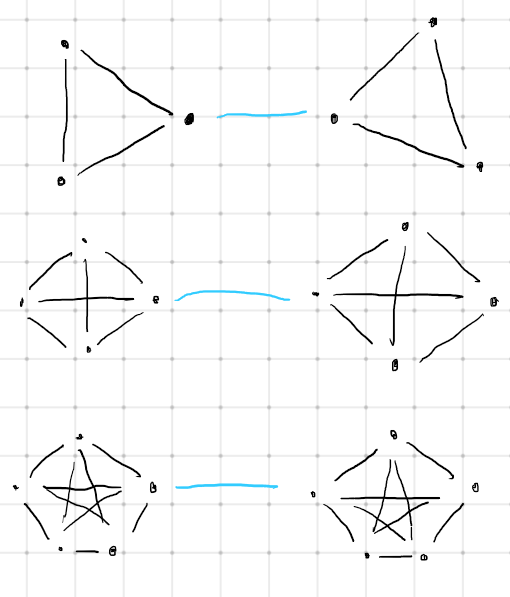
\includegraphics[scale=0.5]{4-1.png}

\end{answer}

\begin{ppart}
    Give an example of a connected graph H with at least 3 edges whose mincut has exactly 1/2 of its vertices on each side of any min-cut. What is the mincut in your graph H? Is the mincut in H unique? Explain your answer

    Now consider the max-cut problem for the graph H. Find one max-cut in your graph, and state the size of the maxcut.
\end{ppart}

\begin{answer}
    With the same graph as the previous answer, we can have a graph that fits the requirements. It's mincut with the blue line, and each side will always have the same amount of vertices.

    The maxcut of the graph is as follows, and has a cut of size 12. 

    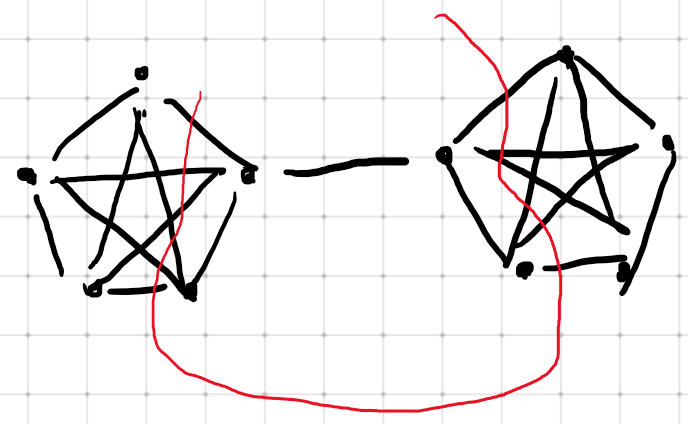
\includegraphics[scale=0.5]{4-3.png}
\end{answer}

\newpage

\begin{problem}
    Let M be an n by n matrix of 0's and 1's. M(i, j) is the entry in row i column j.
    
    We call M rearrangeable if there is a sequence of row switches and column switches of M which result in all 1's along the diagonal of the matrix.

    \begin{ppart}
        Give an example of a 3 x 3 M which is not rearrangeable but which has at least one 1 in each every row and every column.
    \end{ppart}
    
    \begin{answer}
$
        \begin{bmatrix}
            1 & 1 & 1 \\
            0 & 0 & 1 \\
            0 & 0 & 1
        \end{bmatrix}
$
    \end{answer}

    \begin{ppart}
        Write an efficient algorithm to decide if a matrix M is rearrangeable.
    \end{ppart}

    \begin{answer}
        Create a bipartite graph G = (L,R,E) for a matrix M of size n x n, create n vertices in L, where each vertices $l_i$ represents the $i^{th}$ row in the matrix, and n vertices in R.

        If row i contains a 1 in the $j^{th}$ column, add an edge between $l_i$ and $r_j$ into E.

        Calculate if G contains a perfect matching between L and R, we could use Hopcroft-Karp algorithm or similar


        \begin{proof}
            If we have n vectors, whereas the first vector has a 1 in the 1st column, second vector has a 1 in the 2nd column... and so on, this forms a matrix with all 1s on it's diagonal. We can define this as a rearrangeable matrix.
            
            Each edge in G to $r_j$ represents that there is a 1 in the $j^{th}$ column for the row. Thus, if we have a perfect matching, that means for each $r_j$, we can uniquely assign a row vector from matrix M that fits its condition, which means that it is rearrangeable as per our definiton.

            \nline

            The transformation requires n steps for each row, therefore it is $\Ocal(n^2)$ and there will be n vectors in L and R and at most $n^2$ in E, so the complexity using Hopcroft-Karp will be $\Ocal(n^{2.5})$, thus the total complexity is $\Ocal(n^{2.5})$

        \end{proof}

    \end{answer}

    \begin{ppart}
        Show how your algorithm works and what answer it gives on the 4 by 4 matrix M:

$
        \begin{bmatrix}
            0 & 1 & 1 & 0 \\
            1 & 0 & 0 & 1 \\
            1 & 0 & 0 & 0 \\
            0 & 1 & 0 & 0
        \end{bmatrix}
$
    \end{ppart}

    \begin{answer}
        This matrix can be transformed into the following graph (1), which has the red lines as a possible perfect matching. Thus it is rearrangeable
        
        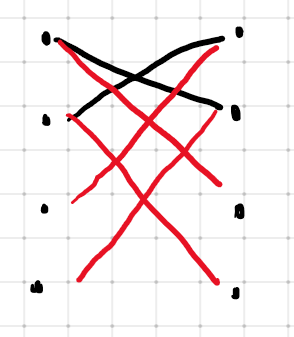
\includegraphics[scale=0.5]{5-3.png}
    \end{answer}
        
\end{problem}
\end{document}
